\documentclass[11pt]{article}
\usepackage{indentfirst}
\usepackage{listings}
\usepackage{graphicx}

\begin{document}
\title{\vspace{-5cm}Sound and music description, revisited}
\date{February 2020}
\author{Tomás Bilal Iaquinta}

\maketitle
\hrulefill
\pagenumbering{arabic}

\section*{Question 1}

As a first step 10 instruments were selected among the suggested ones, those were: \textbf{acoustic guitar, violin, trumpet, naobo, cello, snare drum, transverse flute, bassoon, clarinet, xiaoluo}. These represent different families of instruments: percussive, stringed and wind.\vspace{8pt}

The code was modified for having high quality downloads as suggested. After reviewing the \textit{Freesound.org} web, a dictionary in Python was created to include each instrument as a key, along with tags for each one, that point to one note/stroke sounds. The tags used were mostly \textbf{'single-note'} and \textbf{'1-shot'}. For the snare drum the query text \textbf{'snare\_pearl'} was used since it successfully yielded only single strokes. The selection of the transverse flute was also helpful for obtaining single notes. \vspace{8pt} 

Please refer to the uploaded archives for the specific code used.

\section*{Question 2}

Next step was to try different pair of parameters and watching the scatter plot for all sounds, after a several tries certain parameters were extracted for the k-means algorithm. \vspace{8pt} 

Again, after trying different combinations a \textbf{68.5\%} which will be our \textbf{baseline clustering performance}. The parameters used were:


\begin{itemize}
	\item \textbf{Low-level dissonance mean}
	\item \textbf{Log attack time mean}
	\item \textbf{Low-level MFCC mean} (3rd coefficient)
\end{itemize}

\section*{Question 3}

For this question we need to first update the \textbf{essentia} package, which was done via the terminal by: \begin{verbatim} python -m pip install --upgrade essentia 
\end{verbatim}

\vspace{8pt} 
Then, a function called \texttt{computeEnergy()} was created, in order to compute the \textbf{energy} and \textbf{STFT} of the input audio file for each frame of length $H$. Plots were computed for the energy of some instruments, in order to look for a threshold candidate to not consider non-desirable pieces of the audio (i.e. silence). Then, an energy  \texttt{threshold = 0.002} was selected. Another function called \texttt{plotSampleEnergy()} was created to plot sample sounds energies along with the threshold was also created. Yielding for example what is seen in Figure \ref{fig:energy1}.

\begin{figure}[h]
  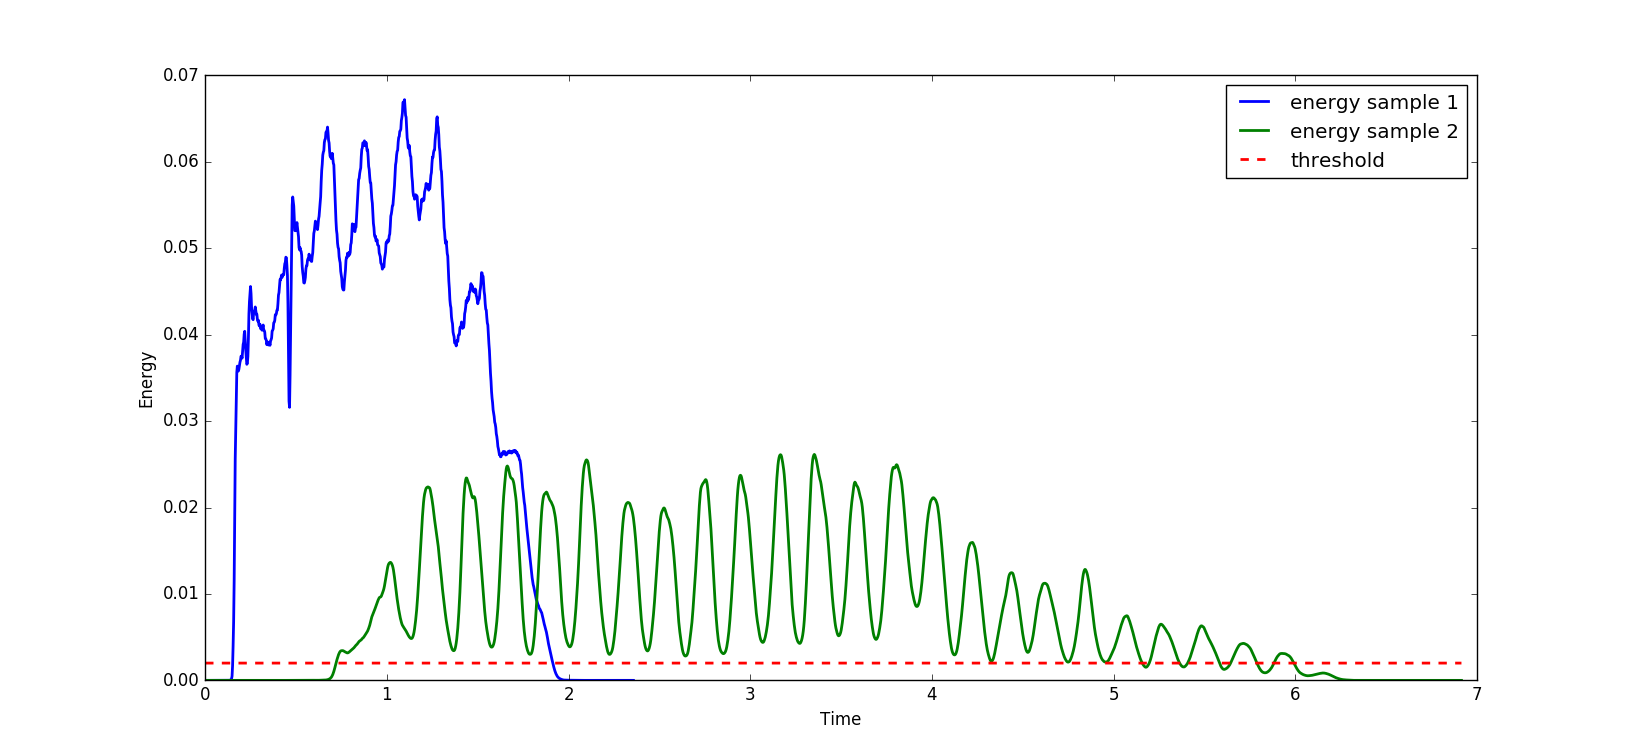
\includegraphics[width=\linewidth]{figure_1.png}
  \caption{Energy of sample sounds and selected energy threshold.}
  \label{fig:energy1}
\end{figure}

So, to calculate the parameters the code is modified to compute only the part of the audio in between the first and the last frames where the energy is superior to the energy threshold. This is done with the function \texttt{frameEnergyThreshold()} which calls the previously introduced one and returns frame by frame the input audio where the condition stated above is true.

\vspace{8pt} 
Then, the \texttt{LowLevelSpectralExtractor()} function was used to extract a multitude of parameters for each input audio frame. These parameters are related to several spectral characteristics, which are seen as adequate to improve the clustering efficiency. Only some of the extracted parameters will be used, while other are discarded.

\vspace{8pt} 
All selected parameters are computed with the \texttt{calculateParameters()} function, and then by running the \texttt{addParameters()} function, all the \texttt{.json} files downloaded from \texttt{Freesound.org} are edited, to include the new parameters calculated. The \texttt{soundAnalysis.py} is updated for their clustering analysis.

\vspace{8pt} 
Repeating what was done on Question 2, different scatter plots are viewed, and the clustering performance for some combinations is computed.

\vspace{8pt}
Finally, with the parameters indicated below a \textbf{75\%} \textbf{clustering performance} is obtained, showing an improvement on the previously obtained one. These are:

\begin{itemize}
	\item \textbf{Low-level MFCC mean} (2nd coefficient)
	\item \textbf{Low-level MFCC mean} (3rd coefficient)
	\item \textbf{Spectral flatness} [dB]
\end{itemize}

Other shortlisted parameters, which yielded similar accuracy, where: -\textbf{Log attack time}, -\textbf{Low-level spectral contrast} (mean 0, 4, 5), -\textbf{Bark bands skewness}, -\textbf{Pitch}, -\textbf{Pitch salience}, -\textbf{Spectral complexity}, -\textbf{Spectral energy band}(middle), and -\textbf{Spectral roll-off}.

\vspace{8pt}
Concluding, by adding one of the new parameters in the analysis, and combining with the ones downloaded from the page, the accuracy is improved. For improving the obtained representation one possibility would be to calculate everything again using the \texttt{frameEnergyThreshold()} function.
\hrulefill

\subsection*{Final remarks}

\begin{itemize}
	\item{In the uploaded files you can find all relevant code used for the assignment. If you insert you API key in the \texttt{assignment.py} file, you can run all the code as was performed.}
	\item{Be aware that the execution of the mentioned file, and of the function \texttt{addParameters()} takes a considerable amount of time, since it makes a very long calculation.}
	\item{By including more than 3 parameters a better performance will be obtained, however since so many parameters are available, obtaining a good performance with only this quantity was the objective.}
\end{itemize}

\end{document}
